\setcounter{section}{2}

\section{Lecture 3:Jan 25}


\subsection*{Last time}
\begin{itemize}
\item Git
\item Linear algebra: vector and vector space, rank of a matrix
\end{itemize}


\subsection*{Today}
\begin{itemize}
\item Column space and Nullspace (JM Appendix A)
\item Simple Linear Regression (JF Chapter 5)
\end{itemize}

\subsection*{Column space}

{\it Definition:} The column space of a matrix, denoted by $\columnSpace{\vecc{A}}$ is the vector space spanned by the columns of the matrix, that is,
$$
\columnSpace{\vecc{A}} = \{\vecc{x} : \mbox{ there exists a vector } \vecc{c} \mbox{ such that } \vecc{x}=\vecc{Ac} \}.
$$

This means that if $\vecc{x} \in \columnSpace{\vecc{A}}$, we can find coefficients $c_j$ such that
$$
\vecc{x} = \sum\limits_{j}c_j \vecc{a}^{(j)}
$$
where $\vecc{a}^{(j)} = \vecc{A}_{\cdot j}$ denotes the j$^{th}$ column of matrix $\vecc{A}$.

\begin{itemize}
  \item The column space of a matrix consists of all vectors formed by multiplying that matrix by any vector.
  \item The number of basis vectors for $\columnSpace{\vecc{A}}$ is then the number of linearly independent columns of the matrix $\vecc{A}$, and so, $\dimm\left(\columnSpace{\vecc{A}}\right) = \rank(\vecc{A})$.
  \item The dimension of a space is the number of vectors in its basis.
\end{itemize}

\subsubsection*{Example A.2}

Let $\vecc{A} = \left[ \begin{array}{ccc} 1 & 1 & -3 \\1 & 2 & -1 \\1 & 3 & 1 \\1 & 4 & 3 \\ \end{array} \right]$ and $\vecc{c} = \left[ \begin{array}{c} 5\\4\\3\\ \end{array} \right]$.   Show that $\vecc{Ac}$ is a linear combination of columns in $\vecc{A}$.

{\it solution:}
$$
\vecc{Ac} = \left[ \begin{array}{c} 1 \times 5 + 1 \times 4 + (-3) \times 3 \\ 1 \times 5 + 2 \times 4 + (-1) \times 3 \\ 1 \times 5 + 3 \times 4 + 1 \times 3 \\ 1 \times 5 + 4 \times 4 + 3 \times 3 \\ \end{array}\right] = \left[ \begin{array}{c} 0 \\ 10 \\ 20\\ 30\\ \end{array} \right].
$$
You could recognize that 
$$
\vecc{Ac} = 5 \times \left[ \begin{array}{c} 1 \\ 1 \\ 1 \\ 1\\ \end{array} \right] + 4 \times \left[ \begin{array}{c} 1 \\ 2 \\ 3 \\ 4\\ \end{array} \right] + 3 \times \left[ \begin{array}{c} -3 \\ -1 \\ 1 \\ 3\\ \end{array} \right] = 5 \vecc{a}^{(1)} + 4 \vecc{a}^{(2)} + 3 \vecc{a}^{(3)}  = \left[ \begin{array}{c} 0 \\ 10 \\ 20\\ 30\\ \end{array} \right].
$$

\subsubsection*{Result A.1}
$\rank(\vecc{AB}) \le \min(\rank(\vecc{A}), \rank(\vecc{B}))$.

{\it proof:} Each column of $\vecc{AB}$ is a linear combination of columns of $\vecc{A}$ (i.e.~$(\vecc{AB})_{\cdot j} = \vecc{A} \vecc{b}^{(j)}$), 
so the number of linearly independent columns of $\vecc{AB}$ cannot be greater than that of $A$.  Similarly, $\rank(\vecc{AB}) = \rank(\vecc{B}\transpose\vecc{A}\transpose)$, the same argument gives $\rank(\vecc{B}\transpose)$ as an upper bound.


\subsubsection*{Result A.2}
\begin{itemize}
 \item (a) If $\vecc{A} = \vecc{BC}$, then $\columnSpace{\vecc{A}} \subseteq \columnSpace{\vecc{B}}$.
 \item (b) If $\columnSpace{\vecc{A}} \subseteq \columnSpace{\vecc{B}}$, then there exists a matrix $\vecc{C}$ such that $\vecc{A} = \vecc{BC}$.
\end{itemize}

{\it proof: }
For (a), any vector $\vecc{x} \in \columnSpace{\vecc{A}}$ can be written as $\vecc{x} = \vecc{Ad} = \vecc{B(Cd)}$.\\
For (b), $\vecc{A}_{\cdot j} \in \columnSpace{B}$, so that there exists a vector $\vecc{c}^{(j)}$ such that $\vecc{A}_{\cdot j} =  \vecc{B} \vecc{c}^{(j)}$.  The matrix $\vecc{C} = (\vecc{c}^{(1)}, \vecc{c}^{(2)}, \dots, \vecc{c}^{(n)})$ satisfies that $\vecc{A} = \vecc{BC}$.


\subsection*{Null space}

{\it Definition:} The null space of a matrix, denoted by $\Null{\vecc{A}}$, is $\Null{\vecc{A}} = \{\vecc{y} : \vecc{Ay} = \vecc{0}\}$.

\subsubsection*{Result A.3}
If $\vecc{A}$ has full-column rank, then $\Null{\vecc{A}} = \{\vecc{0}\}$.

{\it proof:} Matrix $\vecc{A}$ has full-column rank means its columns are linearly independent, which means that $\vecc{Ac} = \vecc{0}$ implies $\vecc{c} = \vecc{0}$.


\subsubsection*{Theorem A.1}
Assume $\vecc{A} \in \mathbb{R}^{m \times n}$, then $\dimm(\columnSpace{\vecc{A}}) = r$ and $\dimm(\Null{\vecc{A}}) = n - r$, where $r = \rank(\vecc{A})$.

See JM Appendix Theorem A.1 for the proof.\\
Interpretation: ``dimension of column space + dimension of null space = \# columns''\\
{\it Mis}Interpretation: Columns space and null space are orthogonal complement to each other. They are of different orders in general! Next result gives the correct statement.

\newpage

\subsection*{Simple linear regression}

Figure~\ref{fig:weights} shows Davis's data on the measured and reported weight in kilograms of $101$ women who were engaged in regular exercise.
\begin{figure}[H]
\begin{center}
  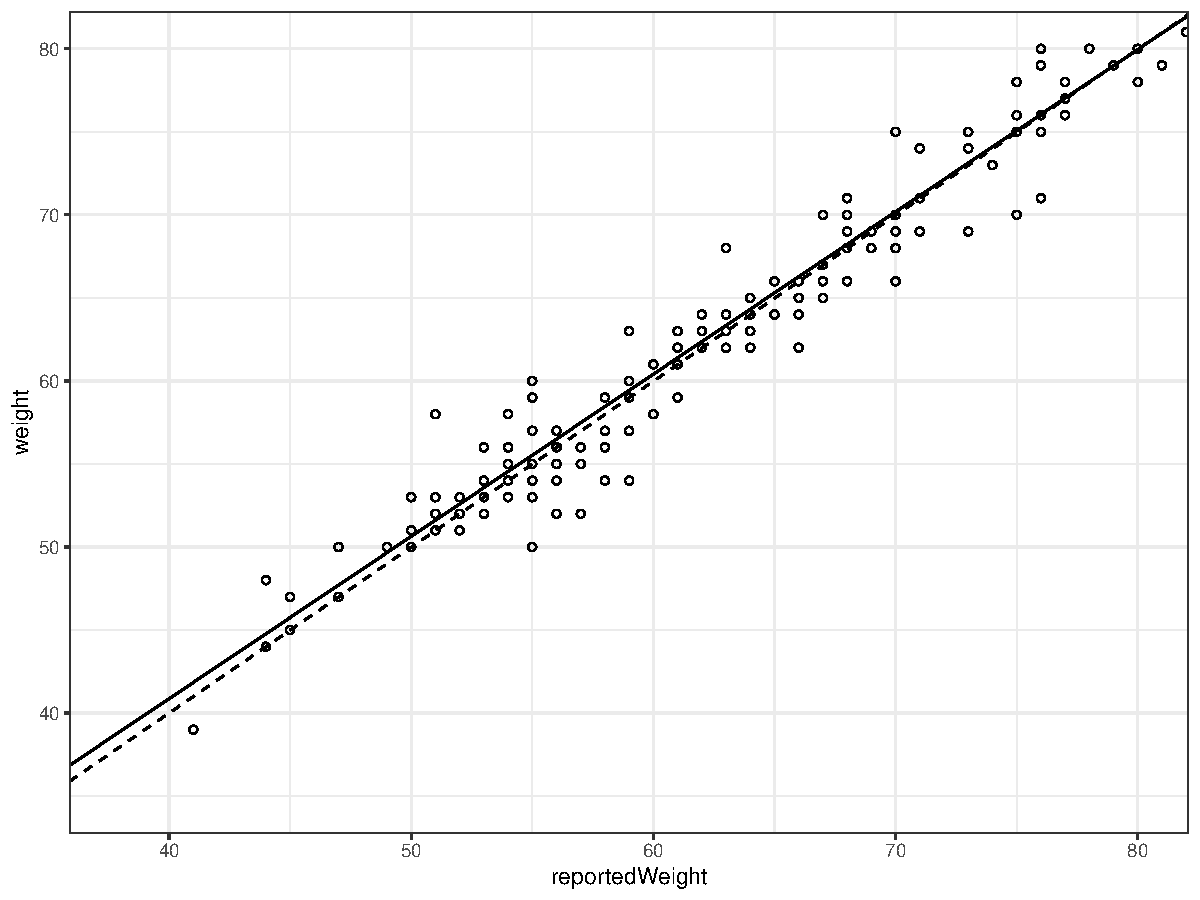
\includegraphics[width=0.8\textwidth]{Lecture3/figure_5_1.pdf}
%  \captionsetup{labelformat=empty}
  \caption{Scatterplot of Davis's data on the measured and reported weight of $101$ women.  The dashed line gives $y = x$.}
  \label{fig:weights}
\end{center}
\end{figure}

It's reasonable to assume that the relationship between measured and reported weight appears to be linear.
Denote:
\begin{itemize}
  \item measured weight by $y_i$: {\bf response variable} or {\bf dependent variable}
  \item reported weight by $x_i$: {\bf predictor variable} or {\bf independent variable}
  \item intercept: $\beta_0$ %= \Expected{y | x = 0
  \item slope: $\beta_1$
  \item residual/error term $\epsilon_i$.
\end{itemize}
%
Then the simple linear regression model writes:
$$
y_i = \beta_0 + \beta_1 x_i + \epsilon_i.
$$
For given $(\hat{\beta}_0, \hat{\beta}_1)$ values, the {\it fitted value} or {\it predicted value} for observation $i$ is:
$$
\hat{y}_i = \hat{\beta}_0 + \hat{\beta}_1 x_i.
$$
%
Therefore, the residual is
$$
\epsilon_i = y_i - \hat{y}_i 
$$

\subsubsection*{Fitting a linear model}

Choose the ``best'' values for $\beta_0, \beta_1$ such that 
$$
SS[E] = \sum\limits_{1}^{n}\left( y_i - (\hat{\beta}_0 + \hat{\beta}_1 x_i) \right)^2 = \sum\limits_{1}^{n}(y_i - \hat{y}_i)^2 = \sum\limits_{1}^{n}\epsilon_i^2
$$
is minimized.
These are {\bf least squares} (LS) estimates:
$$
\begin{array}{l}
\hat{\beta}_0 = \bar{y} - \hat{\beta}_1 \bar{x}\\
\hat{\beta}_1 = \frac{\sum(x_i - \bar{x})(y_i - \bar{y})}{\sum(x_i - \bar{x})^2}.\\
\end{array}
$$

{\it Definition: } The line satisfying the equation
$$
y = \hat{\beta}_0 + \hat{\beta}_1 x
$$
is called the \underline{linear regression} of $y$ on $x$ which is also called the \underline{least squares line}.

For Davis's data, we have
\begin{equation*}
\begin{aligned}
n &= 101 \\
\bar{y} &= \frac{5780}{101} = 57.228\\
\bar{x} &= \frac{5731}{101} = 56.743\\
\sum(x_i - \bar{x})(y_i - \bar{y}) &= 4435.9\\
\sum(x_i - \bar{x})^2 &= 4539.3,\\
\end{aligned}
\end{equation*}
so that
\begin{equation*}
\begin{aligned}
\hat{\beta}_1 &= \frac{4435.9}{4539.3} = 0.97722\\
\hat{\beta}_0 &= 57.228 - 0.97722 \times 56.743 = 1.7776\\
\end{aligned}
\end{equation*}
